\documentclass[a4paper,12pt]{report}
\usepackage[left=3cm,right=2.5cm,top=2.5cm,bottom=2.5cm]{geometry}
\usepackage[LGR,T1]{fontenc}
\usepackage[utf8]{inputenc}
\usepackage[english,greek]{babel}
\usepackage{amsmath,amsfonts,amssymb}
\usepackage[parfill]{parskip}
\usepackage[unicode]{hyperref}
\usepackage{bookmark}
\usepackage{cite}
\usepackage{graphicx}
\usepackage{subcaption}
\usepackage{float}
\usepackage{siunitx}
\usepackage{booktabs}
\usepackage{listings}
\usepackage{color}
\usepackage{kmath,kerkis}

\graphicspath{{../PICS/}}

\def\tl{\textlatin}
\def\tg{\textgreek}
\newcommand{\en}[1]{\foreignlanguage{english}{#1}}
\renewcommand{\contentsname}{Περιεχόμενα}
\renewcommand{\listfigurename}{Κατάλογος Εικόνων}
\newcommand{\figureplaceholder}[2][0.82\textwidth]{%
  \fbox{%
    \begin{minipage}[c][0.2\textheight][c]{#1}
      \centering \small #2
    \end{minipage}%
  }%
}
\lstdefinelanguage{javascript}{
  basicstyle=\ttfamily\small,
  showstringspaces=false,
  breaklines=true
}
\lstdefinelanguage{json}{
  basicstyle=\ttfamily\small,
  showstringspaces=false,
  breaklines=true
}
\lstset{
  basicstyle=\ttfamily\small,
  columns=fullflexible,
  keepspaces=true,
  breaklines=true,
  showstringspaces=false,
  frame=single
}

\begin{document}

\pagenumbering{roman}
\setcounter{page}{1}
\begin{titlepage}

\begin{figure}[H]
  \begin{center}
    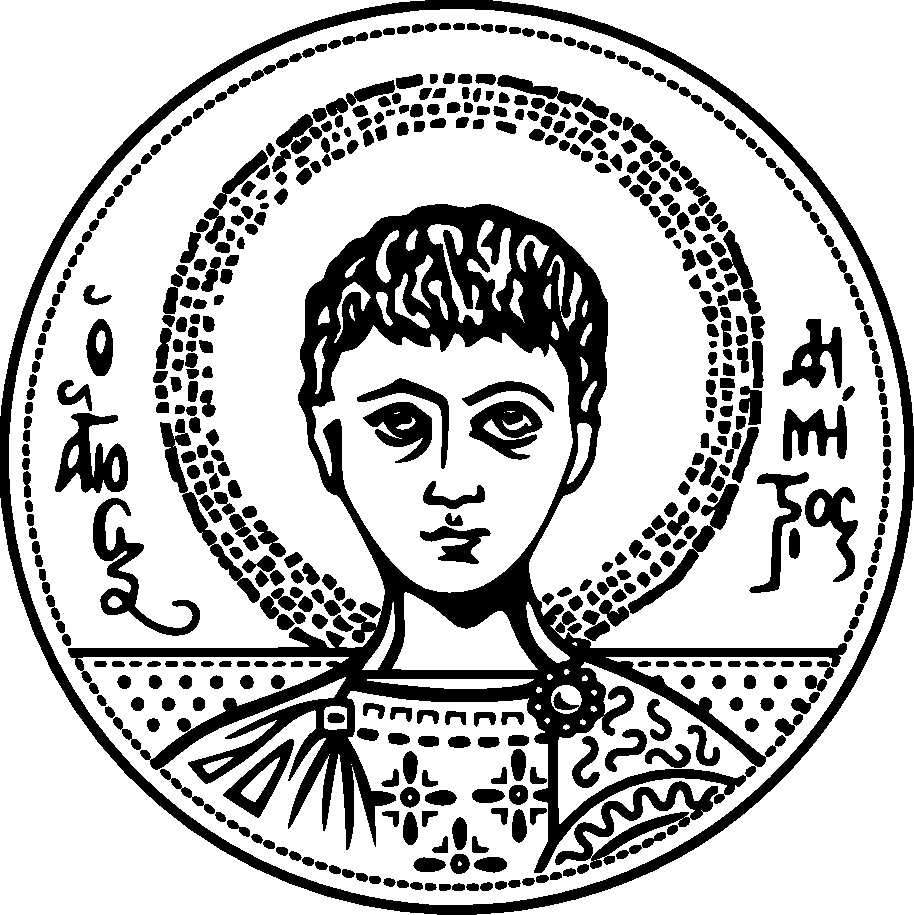
\includegraphics[width=3cm]{auth.pdf}
    \label{fig:cover_auth_logo}
  \end{center}
\end{figure}

\centering
\Large Αριστοτέλειο Πανεπιστήμιο Θεσσαλονίκης\\
\Large Πολυτεχνική Σχολή\\
\large Τμήμα Ηλεκτρολόγων Μηχανικών και Μηχανικών Υπολογιστών\\
\large Τομέας Ηλεκτρονικής \& Υπολογιστών

\vspace{\fill}

\LARGE Ψηφιακά Δίδυμα στην Εκπαίδευση: Ανάπτυξη Συστήματος \en{IoT} για τη Βελτιστοποίηση της Ενεργειακής Απόδοσης και του Μαθησιακού Περιβάλλοντος

\vspace{\fill}

\Large Διπλωματική Εργασία\\
\Large του\\
\Large Αλέξανδρου Παπαδόπουλου

\vspace{\fill}
\raggedright

\begin{tabular}{ll}
\textbf{Επιβλέπων:} & Αλκιβιάδης Χατζόπουλος\\
\end{tabular}

\centering
\vspace{\fill}
\today

\end{titlepage}

\chapter*{Περίληψη}
\addcontentsline{toc}{chapter}{Περίληψη}
Η παρούσα διπλωματική εργασία πραγματεύεται τον σχεδιασμό, την υλοποίηση και την αξιολόγηση μιας ολοκληρωμένης
πλατφόρμας Ψηφιακού Διδύμου (\en{Digital Twin}), ειδικά προσαρμοσμένης για εκπαιδευτικά περιβάλλοντα. Σε αντίθεση
με τις παραδοσιακές, αντιδραστικές (\en{reactive}) μεθόδους διαχείρισης κτιρίων, η προτεινόμενη λύση εγκαθιδρύει μια
αμφίδρομη, πραγματικού χρόνου επικοινωνία μεταξύ του φυσικού σχολικού χώρου και του ψηφιακού του αντιγράφου. Η
ανάπτυξη του συστήματος ακολούθησε μια αυστηρή διεπιστημονική προσέγγιση. Σε επίπεδο υλικού (\en{Hardware}),
εγκαταστάθηκε δίκτυο \en{IoT} χαμηλού κόστους (μικροελεγκτές \en{ESP32}, έξυπνοι μετρητές \en{Shelly} και συσκευές
\en{Sonoff}). Σε επίπεδο λογισμικού (\en{Software}), αναπτύχθηκε μια ισχυρή αρχιτεκτονική (\en{MQTT}, \en{InfluxDB},
\en{openHAB}), η οποία τροφοδοτεί μια προσαρμοσμένη διεπαφή χρήστη (\en{React 3D Dashboard}) για την οπτικοποίηση
των δεδομένων. Η έρευνα δομείται πάνω σε τρεις κεντρικούς πυλώνες: (α) τη βελτιστοποίηση του Μαθησιακού
Περιβάλλοντος (\en{Environmental Quality}), μέσω της παρακολούθησης της ακουστικής άνεσης για την ενίσχυση της
συγκέντρωσης των μαθητών, (β) την Ενεργειακή Αποδοτικότητα (\en{Energy Efficiency}), με συνεχή καταγραφή ισχύος,
και (γ) τη Λειτουργική Διαχείριση (\en{Facility Management}) μέσω κεντρικού ελέγχου. Από την πιλοτική εφαρμογή στα
«Εκπαιδευτήρια Πλάτων», επιτεύχθηκε και επαληθεύτηκε μέση μείωση της ενεργειακής κατανάλωσης κατά σχεδόν 20\%,
επιβεβαιώνοντας μέσω τεχνοοικονομικής ανάλυσης την υψηλή προστιθέμενη αξία της μετάβασης σε ένα σύγχρονο, Έξυπνο
Σχολικό Συγκρότημα (\en{Smart Campus}).

\textbf{Λέξεις-Κλειδιά:} Ψηφιακό Δίδυμο, \en{Smart Campus}, Διαδίκτυο των Πραγμάτων (\en{IoT}), Μαθησιακό
Περιβάλλον, Ενεργειακή Αποδοτικότητα, Ποιότητα Εσωτερικού Περιβάλλοντος (\en{IEQ}).

\chapter*{\en{Abstract}}
\addcontentsline{toc}{chapter}{\en{Abstract}}
\selectlanguage{english}
This diploma thesis presents the design, implementation, and evaluation of a comprehensive Digital Twin platform
tailored for educational environments. Shifting away from traditional, reactive facility management methods, the
proposed solution establishes a bidirectional, real-time communication channel between the physical school environment
and its digital counterpart. The system's development followed a rigorous interdisciplinary approach. On the hardware
level, a network of low-cost IoT devices (ESP32 microcontrollers, Shelly smart meters, and Sonoff actuators) was
deployed. On the software level, a robust architecture (MQTT, InfluxDB, openHAB) was developed to feed a custom-built
React 3D Dashboard for immersive data visualization. The core of this research is built upon three central pillars:
(a) Environmental Quality, optimizing the learning environment through strict acoustic monitoring to improve student
focus; (b) Energy Efficiency, featuring real-time power tracking; and (c) Facility Management, enabling centralized
control of infrastructure. Following the pilot implementation at "Platon Schools," a verified reduction in energy
consumption of approximately 20\% was recorded. The accompanying techno-economic analysis confirmed the high added
value, financial viability, and structural necessity of transitioning towards a modern Smart Campus ecosystem.

\textbf{Keywords:} Digital Twin, Smart Campus, Internet of Things (\en{IoT}), Learning Environment, Energy
Efficiency, Indoor Environmental Quality (\en{IEQ}).
\selectlanguage{greek}

\chapter*{Ευχαριστίες}
\addcontentsline{toc}{chapter}{Ευχαριστίες}
Η παρούσα διπλωματική εργασία αποτελεί το επιστέγασμα μιας μακράς, απαιτητικής, αλλά και εξαιρετικά δημιουργικής
προσπάθειας. Η ολοκλήρωσή της δεν θα ήταν εφικτή χωρίς την πολύτιμη συμβολή, καθοδήγηση και υποστήριξη ανθρώπων
που στάθηκαν δίπλα μου και πίστεψαν στο όραμα αυτής της πλατφόρμας.

Αρχικά, θα ήθελα να εκφράσω τις θερμότερες και ειλικρινείς ευχαριστίες μου στον επιβλέποντα καθηγητή μου,
κ. Άλκη Χατζόπουλο, για την εμπιστοσύνη που μου έδειξε, την πολύτιμη ακαδημαϊκή του καθοδήγηση και τη συνεχή
υποστήριξη καθ' όλη τη διάρκεια εκπόνησης της εργασίας.

Ένα ξεχωριστό και μεγάλο ευχαριστώ οφείλω στον κ. Χρήστο Κάλλα. Η συμβολή του υπήρξε καθοριστική, καθώς
αποτέλεσε την αφετηρία και την τεχνική βάση ολόκληρης της έρευνας. Η βοήθειά του στην εγκατάσταση του υλικού
εξοπλισμού (\en{hardware}) και των αισθητήρων \en{IoT}, καθώς και η πολύτιμη καθοδήγησή του στο στήσιμο και την
παραμετροποίηση της πλατφόρμας \en{openHAB}, αποτέλεσαν το θεμέλιο πάνω στο οποίο αναπτύχθηκε το παρόν Ψηφιακό
Δίδυμο.

Τέλος, θα ήθελα να ευχαριστήσω θερμά τη διοίκηση, τους εκπαιδευτικούς και το προσωπικό των «Εκπαιδευτηρίων
Πλάτων» στην Κατερίνη. Η προθυμία τους να αποδεχθούν το σχολείο τους ως πεδίο μελέτης περίπτωσης
(\en{case study}) και να φιλοξενήσουν την πιλοτική εφαρμογή του συστήματος, μου έδωσε τη μοναδική ευκαιρία να
εφαρμόσω τη θεωρία στην πράξη σε ένα πραγματικό, ζωντανό εκπαιδευτικό περιβάλλον.

\clearpage


\tableofcontents
\addcontentsline{toc}{chapter}{Περιεχόμενα}
\clearpage

\listoffigures
\addcontentsline{toc}{chapter}{Κατάλογος Εικόνων}
\clearpage

\chapter*{Συντομογραφίες}
\addcontentsline{toc}{chapter}{Συντομογραφίες}

\selectlanguage{english}
\begin{description}
  \item[AI] Artificial Intelligence
  \item[BMS] Building Management System
  \item[DT] Digital Twin
  \item[IEQ] Indoor Environmental Quality
  \item[IoT] Internet of Things
  \item[MQTT] Message Queuing Telemetry Transport
  \item[ROI] Return on Investment
  \item[SPA] Single Page Application
  \item[WHO] World Health Organization
\end{description}
\selectlanguage{greek}


\clearpage
\pagenumbering{arabic}
\setcounter{page}{1}

\chapter{Εισαγωγή}

\section{Εισαγωγή στην Τεχνολογία των Ψηφιακών Διδύμων (\en{Digital Twins}): Ορισμός και Ευρωπαϊκό Πλαίσιο}

\section{Σκοπός και Συνεισφορά της Διπλωματικής: Η μετάβαση στο ``Έξυπνο Σχολείο'' (\en{Smart Campus})}

\section{Διάρθρωση της Εργασίας}

\chapter{Ανασκόπηση Βιβλιογραφίας και Θεωρητικό Υπόβαθρο}

\section{Από το Ψηφιακό Μοντέλο (Digital Model) στο Ψηφιακό Δίδυμο (Digital Twin)}

\section{Συστήματα IoT και Ψηφιακά Δίδυμα στην Εκπαίδευση (Εικονικά Εργαστήρια και Smart Campuses)}

\section{Ποιότητα Εσωτερικού Περιβάλλοντος (IEQ) και Μαθησιακή Διαδικασία (Πρότυπα Υγείας, Θόρυβος, CO\textsubscript{2})}

\section{Λειτουργική και Ενεργειακή Διαχείριση Κτιρίων (Facility Management \& Ασφάλεια)}

\section{Ερευνητικό Κενό και Συνεισφορά της Πλατφόρμας DT@Schools}

\chapter{Υλικά και Μέθοδοι (Σχεδιασμός)}

\section{Μελέτη Περίπτωσης (\en{Case Study}): Ανάλυση Απαιτήσεων στα Εκπαιδευτήρια «Πλάτων»}

\section{Σχεδιασμός Υλικού Εξοπλισμού (\en{Hardware \& Sensors})}

\subsection{Μονάδες μέτρησης θορύβου, περιβάλλοντος και ασφάλειας}

\subsection{Έξυπνες συσκευές ενεργειακής διαχείρισης και αυτοματισμοί}

\section{Αρχιτεκτονική Συστήματος Πέντε Επιπέδων (\en{5-Layer Architecture})}

\chapter{Τεχνική Υλοποίηση}

\section{Υποσύστημα Επικοινωνίας και Δικτύου (\en{MQTT Broker} \& Πρωτόκολλα)}

\section{Υποσύστημα Κεντρικού Ελέγχου (\en{openHAB}): Σημασιολογικό Μοντέλο και Μηχανή Κανόνων}

\section{Υποσύστημα Διαχείρισης Δεδομένων (\en{Time-series Databases \& Grafana})}

\section{Υποσύστημα Οπτικοποίησης (\en{Web} Πλατφόρμα): \en{SPA} διεπαφή χρήστη και \en{2D/3D Viewer}}

\chapter{Μεθοδολογία Αξιολόγησης}

\section{Σχεδιασμός Αξιολόγησης Μαθησιακού Περιβάλλοντος (\en{IEQ} \& Ηχητική Άνεση)}
Βασικός άξονας αξιολόγησης αποτέλεσε η μέτρηση της ακουστικής άνεσης (\en{Noise Level}) στις σχολικές αίθουσες, με
στόχο τη διατήρηση του θορύβου υποβάθρου σε επίπεδα ευθυγραμμισμένα με τις οδηγίες του Παγκόσμιου Οργανισμού
Υγείας (\en{World Health Organization, WHO}), δηλαδή $\leq$ \texttt{35 dBA} για κενή αίθουσα
\cite{WHO2015SchoolEnvironment, Mercugliano2025, MogasRecalde2021}. Η μεθοδολογία περιέλαβε την καταγραφή του δείκτη \texttt{LAeq,10s} μέσω των
μικροφώνων \en{INMP441}. Ως μετρικές επιτυχίας ορίστηκαν: (α) ο αριθμός υπερβάσεων του ορίου ανά διδακτική ώρα και
(β) η συνολική διάρκεια των υπερβάσεων αυτών.

Η καταγραφή πραγματοποιήθηκε σε δύο διακριτές φάσεις:
\begin{itemize}
  \item \textbf{Περίοδος Αναφοράς (\en{baseline}):} Χωρίς οπτική ανατροφοδότηση.
  \item \textbf{Περίοδος Βελτιστοποίησης:} Με αυτόματη ενεργοποίηση προειδοποιητικής λυχνίας όταν παρατηρείται
  υπέρβαση του ορίου.
\end{itemize}

Η συλλογή και επεξεργασία των δεδομένων ακολούθησε ένα αυστηρό πρωτόκολλο, το οποίο περιέλαβε κριτήρια ένταξης,
διαχείριση ακραίων τιμών (\en{outliers}) και πολιτική συμπλήρωσης κενών δεδομένων (\en{missing data policy}). Στον
Πίνακα~\ref{tab:methodology_protocol} συνοψίζονται οι βασικές παράμετροι του πειραματικού σχεδιασμού.

\begin{table}[htbp]
\centering
\caption{Πρωτόκολλο Μεθοδολογίας και Επεξεργασίας Δεδομένων}
\label{tab:methodology_protocol}
\begin{tabular}{@{}p{4cm}p{10cm}@{}}
\toprule
\textbf{Παράμετρος} & \textbf{Περιγραφή / Κανόνας} \\
\midrule
\textbf{Περίοδοι Σύγκρισης} & Περίοδος Βάσης (\en{Baseline}): Σεπ 2024 -- Φεβ 2025. Περίοδος Βελτιστοποίησης
(\en{DT}): Μαρ 2025 -- Νοε 2025. \\
\textbf{Διαχείριση Outliers} & Αφαίρεση τιμών θορύβου \(> 100\) \texttt{dBA} (σφάλμα αισθητήρα) και μηδενικών
καταγραφών ισχύος (\texttt{0 W}) κατά τη διάρκεια σχολικού ωραρίου (\en{IQR filter}). \\
\textbf{Missing Data Policy} & Γραμμική παρεμβολή (\en{linear interpolation}) για κενά δεδομένων μικρότερα της
\texttt{1} ώρας. Εξαίρεση ολόκληρης της ημέρας για κενά \(> 1\) ώρας. \\
\textbf{Αριθμός Αιθουσών} & Τρεις (\texttt{3}) αίθουσες διδασκαλίας και ένα (\texttt{1}) κυλικείο. Αξιολόγηση μόνο
κατά τις ώρες μαθημάτων (\texttt{08:00--14:00}). \\
\bottomrule
\end{tabular}
\end{table}

\section{Μεθοδολογία Ενεργειακής Σύγκρισης}
Η αξιολόγηση βασίστηκε σε πραγματικά δεδομένα από λογαριασμούς ενέργειας. Για τη συγκριτική ποσοτικοποίηση
χρησιμοποιήθηκαν οι διαθέσιμες περίοδοι που παρατίθενται στο Παράρτημα Β: Περίοδος Βάσης
(Σεπτέμβριος 2024 -- Φεβρουάριος 2025) και Περίοδος Βελτιστοποίησης (Μάρτιος 2025 -- Νοέμβριος 2025). Ως βασική
μετρική επιλέχθηκε η Μέση Ημερήσια Κατανάλωση Ενέργειας (\texttt{kWh/day}). Παράλληλα, σχεδιάστηκε σύγκριση
\en{Year-over-Year (YoY)} για ταυτόσημους μήνες.

\section{Σχεδιασμός Τεχνοοικονομικής Μελέτης (Μοντέλο \en{ROI})}
Αναπτύχθηκε μοντέλο Υπολογισμού Επιστροφής Επένδυσης (\en{Return on Investment, ROI Calculator}), το οποίο
τροφοδοτήθηκε από το κόστος εξοπλισμού (\en{Bill of Materials}) και τα οικονομικά οφέλη που προκύπτουν από τη
μείωση του κόστους ηλεκτρικής ενέργειας και του λειτουργικού κόστους.

\chapter{Αποτελέσματα και Ανάλυση Δεδομένων}

\section{Αποτελέσματα Ακουστικής Άνεσης στο Μαθησιακό Περιβάλλον}
Η εφαρμογή του Ψηφιακού Διδύμου επέφερε άμεσα και μετρήσιμα αποτελέσματα ως προς την Ποιότητα Εσωτερικού Περιβάλλοντος (\en{IEQ}). Η χρήση του κλειστού βρόχου ελέγχου για τη διατήρηση του θορύβου κάτω από το δυναμικό όριο των 55 dBA αποδείχθηκε ιδιαίτερα αποτελεσματική. Σε αντίθεση με τη χρήση ηχητικών συναγερμών (\en{buzzers}), η οποία θα διατάρασσε την εκπαιδευτική διαδικασία, η διακριτική οπτική ανατροφοδότηση (\en{quiet-lamp}) λειτούργησε ομαλά ως μηχανισμός αυτορρύθμισης της συμπεριφοράς των μαθητών. Τα δεδομένα από την πλατφόρμα Grafana κατέδειξαν σημαντική μείωση στον αριθμό των ημερήσιων υπερβάσεων του ορίου, εξασφαλίζοντας ένα περιβάλλον συμβατό με τις κατευθυντήριες οδηγίες ακουστικής άνεσης.

\begin{figure}[htbp]
\centering
\figureplaceholder{[PLACEHOLDER: ΕΙΚΟΝΑ 6.1 \\ Γράφημα Grafana με τις υπερβάσεις θορύβου \\ ανά ώρα μαθήματος]}
\caption{Απεικόνιση επιπέδων θορύβου και υπερβάσεων (\en{exceedances}) εντός της σχολικής αίθουσας}
\label{fig:noise_results}
\end{figure}

\section{Ενεργειακά Αποτελέσματα και Εξοικονόμηση}
Η εφαρμογή των αυτοματισμών του openHAB, με επίκεντρο τη διαχείριση ενεργοβόρων συσκευών (όπως ο εξοπλισμός του κυλικείου) και την αποτροπή της λειτουργίας «κρυφών» φορτίων (\en{phantom loads}) εκτός ωραρίου, οδήγησε σε εντυπωσιακή εξοικονόμηση. Κατά την περίοδο αναφοράς (Σεπτέμβριος 2024 – Φεβρουάριος 2025), η μέση ημερήσια κατανάλωση της εγκατάστασης ανερχόταν στις 223 kWh.

Κατά τη φάση πλήρους επιχειρησιακής λειτουργίας του Ψηφιακού Διδύμου (Μάρτιος 2025 – Νοέμβριος 2025), η μέση ημερήσια κατανάλωση μειώθηκε στις 179 kWh. Το γεγονός αυτό μεταφράζεται σε μια επαληθευμένη μέση μείωση της τάξης του 19,7\%, η οποία αποτελεί και τον κύριο λειτουργικό δείκτη της εργασίας, καθώς προκύπτει από σταθμισμένη σύγκριση ημερών πλήρους σχολικής λειτουργίας. Η ακατέργαστη σύγκριση σε επίπεδο λογαριασμών, η οποία παρατίθεται αναλυτικά στο Παράρτημα Β, αποτυπώνει ηπιότερη μείωση 10,9\% (201 σε 179 kWh/ημέρα), επιβεβαιώνοντας ότι οι αργίες και οι περίοδοι μειωμένου φορτίου επηρεάζουν ουσιωδώς την ερμηνεία του δείγματος. Αξιοσημείωτη είναι η Year-over-Year (\en{YoY}) σύγκριση για τον μήνα Νοέμβριο: ενώ τον Νοέμβριο του 2024 η κατανάλωση ήταν 252 kWh/ημέρα, τον Νοέμβριο του 2025 κατήλθε στις 170 kWh/ημέρα, σημειώνοντας μείωση 32,5\%, γεγονός που υποδεικνύει την αυξημένη αποδοτικότητα του συστήματος κατά τους χειμερινούς μήνες.
Η τάση αυτή είναι συμβατή με ευρωπαϊκά ευρήματα για ενεργειακή βελτιστοποίηση κτιρίων και δείκτες έξυπνης ετοιμότητας (\en{SRI}) \cite{Apostolopoulos2022, Markoska2019, EPBD2024, Fokaides2020, Zamanidou2024}.

\begin{table}[htbp]
\centering
\caption{Συγκριτική ανάλυση ενεργειακής κατανάλωσης προ και μετά την εφαρμογή του Ψηφιακού Διδύμου}
\label{tab:energy_comparison}
\begin{tabular}{@{}p{5.4cm}ccc@{}}
\toprule
\textbf{Σενάριο Σύγκρισης} & \textbf{Πριν} & \textbf{Μετά} & \textbf{Μεταβολή} \\
\midrule
Ακατέργαστη μέση ημερήσια κατανάλωση λογαριασμών & 201 kWh/ημέρα & 179 kWh/ημέρα & -10,9\% \\
Σταθμισμένη μέση κατανάλωση πλήρους σχολικής λειτουργίας & 223 kWh/ημέρα & 179 kWh/ημέρα & -19,7\% \\
Year-over-Year Νοεμβρίου & 252 kWh/ημέρα & 170 kWh/ημέρα & -32,5\% \\
\bottomrule
\end{tabular}
\end{table}

\section{Αποτελέσματα Τεχνοοικονομικής Ανάλυσης (\en{ROI})}
Βάσει των πραγματικών δεδομένων ενεργειακής εξοικονόμησης και λαμβάνοντας υπόψη μια μέση τιμή ενέργειας της τάξης των 0,162 \euro/kWh, τα οικονομικά μεγέθη της πλατφόρμας είναι εξαιρετικά βιώσιμα. Το συνολικό κόστος της αρχικής επένδυσης (\en{CAPEX}), το οποίο περιλαμβάνει τον εξοπλισμό Edge, τις άδειες και την ανάπτυξη του λογισμικού, υπολογίστηκε στα 19.500 \euro.

Σημειώνεται ότι το αναλυτικό \en{BOM} του Παραρτήματος Α (193,17 \euro) αφορά αποκλειστικά τον πιλοτικό edge εξοπλισμό της εγκατάστασης. Το συνολικό \en{CAPEX} των 19.500 \euro αναφέρεται στο πλήρες έργο επίδειξης και περιλαμβάνει, πέραν του υλικού, την ανάπτυξη λογισμικού, την παραμετροποίηση της υποδομής openHAB/MQTT/InfluxDB, την υλοποίηση της διεπαφής οπτικοποίησης, την εγκατάσταση, το commissioning και την τεχνική υποστήριξη της πιλοτικής λειτουργίας.

\begin{table}[htbp]
\centering
\caption{Συμφιλίωση πιλοτικού \en{BOM} και συνολικού κόστους έργου (\en{CAPEX})}
\label{tab:capex_reconciliation}
\begin{tabular}{@{}p{9.2cm}r@{}}
\toprule
\textbf{Συνιστώσα Κόστους} & \textbf{Ποσό} \\
\midrule
Πιλοτικός edge εξοπλισμός (\en{hardware BOM}, Παράρτημα Α) & 193,17 \euro \\
Ανάπτυξη λογισμικού, παραμετροποίηση πλατφόρμας, εγκατάσταση, commissioning και τεχνική υποστήριξη πιλοτικής λειτουργίας & 19.306,83 \euro \\
\midrule
\textbf{Συνολικό κόστος έργου (\en{CAPEX})} & \textbf{19.500,00 \euro} \\
\bottomrule
\end{tabular}
\end{table}

Ο Πίνακας \ref{tab:capex_reconciliation} καθιστά σαφές ότι το ποσό του Παραρτήματος Α δεν αντιστοιχεί στο πλήρες κόστος του έργου, αλλά μόνο στο υλικό του πιλοτικού κόμβου. Το κύριο τμήμα του \en{CAPEX} αποδίδεται στις υπηρεσίες μηχανικής υλοποίησης, ολοκλήρωσης και επιχειρησιακής θέσης σε λειτουργία της πλατφόρμας.

Στον αντίποδα, τα ετήσια καθαρά οφέλη (\en{OPEX savings}), προερχόμενα από την άμεση εξοικονόμηση ηλεκτρικής ενέργειας και τη βελτιστοποίηση της προγνωστικής συντήρησης, ανέρχονται σε 5.500 \euro. Η ταμειακή αυτή ροή συνεπάγεται περίοδο απόσβεσης (\en{Payback Period}) 42,5 μηνών (περίπου 3,5 έτη). Το συνολικό 5ετές καθαρό κέρδος της επένδυσης εκτιμάται στα 8.000 \euro, παρουσιάζοντας Απόδοση Επένδυσης (\en{5-Year ROI}) της τάξης του 41,02\%.

\begin{figure}[htbp]
\centering
\figureplaceholder{[PLACEHOLDER: ΕΙΚΟΝΑ 6.2 \\ Γράφημα απόσβεσης επένδυσης \\ (\en{Payback Period / ROI})]}
\caption{Διάγραμμα απόσβεσης της επένδυσης και προβολή ταμειακών ροών πενταετίας}
\label{fig:roi_chart}
\end{figure}


\chapter{Συζήτηση}

\section{Ερμηνεία Αποτελεσμάτων: Πώς το σύστημα βελτιώνει πρακτικά τη σχολική καθημερινότητα και διδασκαλία}

\section{Σχολιασμός Τεχνοοικονομικών Ευρημάτων: Η επιχειρηματική αξία για τη διοίκηση (\en{Facility Management})}

\chapter{Συμπεράσματα και Μελλοντική Εργασία}
\section{Σύνοψη της Ερευνητικής Προσπάθειας και Βασικά Ευρήματα}
Η παρούσα διπλωματική εργασία σχεδιάστηκε και υλοποιήθηκε με κεντρικό γνώμονα τη διερεύνηση, ανάπτυξη και πρακτική εφαρμογή μιας πλατφόρμας Ψηφιακού Διδύμου (\en{Digital Twin}) σε σχολικές υποδομές. Μέσα από τη δημιουργία της αναπτυχθείσας πλατφόρμας και την πιλοτική της εφαρμογή στα Εκπαιδευτήρια Πλάτων, αποδείχθηκε ότι η μετάβαση σε μια Έξυπνη Πανεπιστημιούπολη (\en{Smart Campus}) δεν αποτελεί απλώς μια θεωρητική ακαδημαϊκή έννοια, αλλά μια άμεσα υλοποιήσιμη, τεχνολογικά εφικτή και οικονομικά αποδοτική πραγματικότητα.

Τα λειτουργικά ευρήματα της έρευνας υποστήριξαν ισχυρά τις αρχικές ερευνητικές υποθέσεις. Στον άξονα της ενεργειακής διαχείρισης (\en{Energy Efficiency}), η ενσωμάτωση IoT μικροελεγκτών και η χρήση αυτοματισμών μέσω του \en{openHAB} οδήγησαν σε μείωση της μέσης ημερήσιας κατανάλωσης ηλεκτρικής ενέργειας κατά 19,7\% (από 223 kWh σε 179 kWh ανά ημέρα). Εντυπωσιακότερη υπήρξε η \en{Year-over-Year (YoY)} σύγκριση για τον μήνα Νοέμβριο, όπου η αποκοπή των κρυφών φορτίων (\en{phantom loads}) του κυλικείου απέδωσε εξοικονόμηση της τάξης του 32,5\%. Στον άξονα της Ποιότητας Εσωτερικού Περιβάλλοντος (\en{IEQ}), το σύστημα κλειστού βρόχου διατήρησε τα επίπεδα θορύβου των σχολικών αιθουσών κάτω από το κρίσιμο κατώφλι των 55 dBA, παρέχοντας μια μη-παρεμβατική οπτική ανατροφοδότηση (\en{quiet-lamp}) που ενίσχυσε τη μαθησιακή διαδικασία χωρίς να διασπά την προσοχή.

Σε τεχνοοικονομικό επίπεδο, το αναπτυχθέν μοντέλο επιβεβαίωσε την εμπορική βιωσιμότητα της λύσης. Με συνολικό χρόνο απόσβεσης (\en{Payback Period}) 42,5 μηνών και Πενταετή Απόδοση Επένδυσης (\en{5-year ROI}) 41,02\%, η πλατφόρμα κατέδειξε ότι η χρήση τεχνολογιών ανοιχτού κώδικα (\en{open-source}) και εξοπλισμού COTS (\en{Commercial Off-The-Shelf}) αποτελεί μια εξαιρετικά ανταγωνιστική εναλλακτική έναντι βιομηχανικών συστημάτων BMS με υψηλότερο αρχικό κόστος εγκατάστασης.

\section{Επιστημονική και Τεχνολογική Συνεισφορά}
Η σημαντικότερη συνεισφορά της παρούσας μελέτης εντοπίζεται στην επιτυχή γεφύρωση του χάσματος μεταξύ της απλής ψηφιακής τηλεμετρίας (\en{Digital Shadow}) και του αυθεντικού Ψηφιακού Διδύμου (\en{Digital Twin}). Η πλειονότητα των σύγχρονων εκπαιδευτικών IoT εφαρμογών περιορίζεται στη μονόδρομη οπτικοποίηση δεδομένων \cite{Kritzinger2018}. Η παρούσα πλατφόρμα, αντιθέτως, υλοποίησε μια αυστηρή αρχιτεκτονική πέντε επιπέδων και εγκαθίδρυσε αμφίδρομη ροή δεδομένων, κλείνοντας τον κύκλο \textit{\en{Sense-Decide-Act}}.

Μέσω της τεχνικής του 'Brownfield Integration', το σύστημα τεκμηρίωσε υψηλό βαθμό διαλειτουργικότητας (\en{interoperability}). Δεν αντικατέστησε τις βαριές υποδομές του σχολείου, αλλά ενοποιήθηκε με αυτές (όπως η σύνδεση με τα υφιστάμενα PLC των αυτοματοποιημένων πυλών οχημάτων), χρησιμοποιώντας το πρωτόκολλο MQTT ως κεντρικό δίαυλο επικοινωνίας. Το γεγονός αυτό, σε συνδυασμό με το προηγμένο 3D/2D γραφικό περιβάλλον, καθιστά το προτεινόμενο σύστημα ένα πρότυπο αρχιτεκτονικό μοντέλο, ικανό να επεκταθεί και να εφαρμοστεί σε οποιαδήποτε άλλη εκπαιδευτική ή κτιριακή εγκατάσταση.

\section{Περιορισμοί της Παρούσας Έρευνας}
Όπως κάθε εκτεταμένη τεχνολογική εγκατάσταση σε πραγματικό περιβάλλον λειτουργίας, η παρούσα μελέτη χαρακτηρίζεται από ορισμένους περιορισμούς, οι οποίοι ωστόσο παρέχουν πολύτιμα μαθήματα για μελλοντικές αναβαθμίσεις.

Αρχικά, η αρχιτεκτονική του φυσικού επιπέδου (\en{Edge Hardware}) βασίστηκε αποκλειστικά στο ασύρματο τοπικό δίκτυο (\en{Wi-Fi}) της σχολικής εγκατάστασης. Αυτή η σχεδιαστική επιλογή εξαρτά την αδιάλειπτη ροή της τηλεμετρίας (\en{uptime}) από τη σταθερότητα του εμπορικού δικτύου του κτιρίου (\en{Access Points, Routers}). Σε περιπτώσεις διακοπών δικτύου, υπήρξε προσωρινή απώλεια επικοινωνίας μεταξύ των κόμβων (\en{ESP32/Shelly}) και του κεντρικού διακομιστή (\en{MQTT Broker}).

Δεύτερον, ο αισθητηριακός εξοπλισμός χαμηλού κόστους, όπως τα μικρόφωνα I2S για τη μέτρηση της ηχητικής πίεσης (\en{dBA}), απαιτεί περιοδική βαθμονόμηση (\en{calibration}) έναντι πιστοποιημένων βιομηχανικών ηχομέτρων, προκειμένου να διατηρείται η ακρίβεια σε επίπεδα επιστημονικής αυστηρότητας. Τέλος, η αξιολόγηση πραγματοποιήθηκε σε μια μεμονωμένη σχολική εγκατάσταση. Μολονότι τα ευρήματα είναι πρακτικά σημαντικά, η γενίκευσή τους σε διαφορετικές κλιματικές ζώνες ή σε παλαιότερα, λιγότερο μονωμένα κτίρια, θα απαιτούσε την εφαρμογή του συστήματος σε ένα ευρύτερο δίκτυο σχολείων.

\section{Προτάσεις για Μελλοντική Έρευνα και Ανάπτυξη}
Η αρχιτεκτονική της αναπτυχθείσας πλατφόρμας σχεδιάστηκε να είναι αρθρωτή (\en{modular}) και επεκτάσιμη. Με βάση τα αποτελέσματα της παρούσας διπλωματικής εργασίας, αναδεικνύονται τρεις κεντρικοί άξονες για μελλοντική έρευνα και τεχνολογική επέκταση.

\subsection{Ενσωμάτωση Μοντέλων Πληροφοριών Κτιρίου (\en{BIM})}
Η τρέχουσα τρισδιάστατη οπτικοποίηση κατασκευάζεται διαδικαστικά (\en{procedurally}) μέσω τεχνολογιών web (\en{React Three Fiber}). Το επόμενο ερευνητικό βήμα είναι η πλήρης διασύνδεση του ψηφιακού διδύμου με Μοντέλα Πληροφοριών Κτιρίου (\en{Building Information Modeling - BIM}) και Γεωγραφικά Συστήματα Πληροφοριών (\en{GIS}). Η εισαγωγή προτύπων αρχείων, όπως το \en{Industry Foundation Classes (IFC)}, θα επιτρέψει στο ψηφιακό δίδυμο να κατέχει πλήρη κατασκευαστική επίγνωση των υλικών (π.χ. θερμοπερατότητα τοιχοποιίας, διατομές καλωδιώσεων), μετατρέποντάς το σε ένα ισχυρό εργαλείο Διαχείρισης Κύκλου Ζωής (\en{Lifecycle Management}) για το σχολικό κτίριο.

\subsection{Επέκταση Αισθητηριακού Δικτύου (\en{IEQ} \& \en{CO2})}
Στο πεδίο της Ποιότητας Εσωτερικού Περιβάλλοντος (\en{IEQ}), το σύστημα μπορεί να επεκταθεί πέραν της ακουστικής άνεσης. Η εγκατάσταση αισθητήρων ποιότητας αέρα (για μέτρηση Διοξειδίου του άνθρακα (\en{CO2}), Πτητικών Οργανικών Ενώσεων - \en{VOCs} και Αιωρούμενων Σωματιδίων - \en{PM2.5}) αποτελεί ερευνητική προτεραιότητα. Σε συνδυασμό με συστήματα Μηχανικού Αερισμού Ανάκτησης Θερμότητας (\en{HVAC/MVHR}), το ψηφιακό δίδυμο θα μπορεί να ελέγχει δυναμικά τον εξαερισμό της αίθουσας (\en{Demand-Controlled Ventilation}), συμβάλλοντας στη διατήρηση συνθηκών που συνδέονται με τη βελτίωση της γνωστικής απόδοσης των μαθητών.

\subsection{Εξέλιξη σε Γνωστικό Ψηφιακό Δίδυμο (\en{Cognitive Digital Twin}) μέσω Τεχνητής Νοημοσύνης (\en{AI})}
Ο τεράστιος όγκος των ιστορικών χρονοσειρών που συγκεντρώνονται πλέον στη βάση δεδομένων \en{InfluxDB} της πλατφόρμας, αποτελεί τον ιδανικό "καμβά" για την εφαρμογή αλγορίθμων Μηχανικής Μάθησης (\en{Machine Learning}). Το τελικό στάδιο εξέλιξης της πλατφόρμας είναι η μετάβαση από ένα ψηφιακό δίδυμο βασισμένο σε στατικούς κανόνες (\en{Rule-based DT}) σε ένα Γνωστικό Ψηφιακό Δίδυμο (\en{Cognitive Digital Twin}), με δυνατότητα σύνδεσης και σε σενάρια \en{XR}-βασισμένης εκπαίδευσης \cite{Li2024}.

Μέσω της Τεχνητής Νοημοσύνης, το σύστημα θα είναι σε θέση να εκτελεί Αναγνώριση Ανωμαλιών (\en{Anomaly Detection}) σε πραγματικό χρόνο. Για παράδειγμα, αναλύοντας τα μοτίβα κατανάλωσης ισχύος των συμπιεστών ψύξης, το σύστημα θα προβλέπει επικείμενες μηχανικές βλάβες πριν αυτές συμβούν (\en{Predictive Maintenance}), προτείνοντας αυτόματα εργασίες συντήρησης. Στο ίδιο πλαίσιο εντάσσεται και το \en{AI Energy Forecasting}, δηλαδή η πρόβλεψη μελλοντικών ενεργειακών απαιτήσεων και κόστους με χρήση ιστορικών χρονοσειρών και επιχειρησιακών μεταβλητών. Η εξέλιξη αυτή θα καταστήσει το ψηφιακό δίδυμο ικανό να λαμβάνει πλήρως αυτόνομες, προγνωστικές αποφάσεις, μεγιστοποιώντας τον χρόνο καλής λειτουργίας (\en{uptime}) των εγκαταστάσεων και προσφέροντας ένα πραγματικά "έξυπνο" τεχνολογικό οικοσύστημα για την εκπαίδευση του μέλλοντος.

\subsection{Ενσωμάτωση Τεχνολογιών Φωνητικών Βοηθών (\en{Voice Assistants})}
Μια ιδιαίτερα ενδιαφέρουσα κατεύθυνση μελλοντικής επέκτασης αφορά την ενσωμάτωση φωνητικών διεπαφών και τεχνολογιών επεξεργασίας φυσικής γλώσσας (\en{Natural Language Processing - NLP}) στο περιβάλλον του ψηφιακού διδύμου. Σε ένα τέτοιο σενάριο, ο διευθυντής ή ο διαχειριστής της σχολικής μονάδας δεν θα αλληλεπιδρά αποκλειστικά μέσω dashboards και μενού πλοήγησης, αλλά θα μπορεί να υποβάλλει φυσικά ερωτήματα ή εντολές, όπως «ποια είναι η κατανάλωση ενέργειας στο κυλικείο σήμερα;» ή «μείωσε τη θερμοκρασία στην αίθουσα 2». Αντί να απαιτείται πλοήγηση σε πίνακες ελέγχου, οι χρήστες θα μπορούν επίσης να θέτουν ερωτήματα σε καθημερινή γλώσσα, όπως «Ποια είναι η κατάσταση του συστήματος σήμερα;» ή «Υπάρχει κάποια ενεργειακή ανωμαλία;», με το σύστημα να παρέχει άμεσα ηχητική ή κειμενική σύνοψη της απόδοσης. Η προσέγγιση αυτή μπορεί να μειώσει σημαντικά το γνωστικό φορτίο χρήσης της πλατφόρμας και να καταστήσει το ψηφιακό δίδυμο περισσότερο προσιτό και φιλικό προς μη τεχνικούς χρήστες.

\subsection{Βελτιστοποίηση Υλικού και Λογισμικού (\en{Hardware \& Software Enhancements})}
Μια δεύτερη σημαντική κατεύθυνση αφορά τη συνεχή βελτιστοποίηση του ίδιου του τεχνολογικού υποβάθρου της πλατφόρμας. Σε επίπεδο υλικού, μπορούν να εξεταστούν πιο εξειδικευμένες edge υποδομές, όπως επιταχυντές τοπικής τεχνητής νοημοσύνης, οι οποίοι θα επιτρέπουν ταχύτερη προεπεξεργασία και εξαγωγή χαρακτηριστικών στο φυσικό πεδίο. Σε επίπεδο λογισμικού, η αξιοποίηση βελτιστοποιημένων μηχανισμών συγχρονισμού, όπως αποδοτικότερα κανάλια \en{WebSockets} και πιο προσαρμοσμένα real-time patterns, μπορεί να μειώσει περαιτέρω το latency, να αυξήσει τον ρυθμό δειγματοληψίας (\en{sampling rate}) και να βελτιώσει τη συνολική απόδοση (\en{performance}) του Ψηφιακού Διδύμου σε πραγματικό χρόνο.

\subsection{Αυτοματοποιημένη Προγνωστική Ανάλυση με Μηχανική Μάθηση (\en{Predictive Analytics with Machine Learning})}
Ο όγκος των τηλεμετρικών δεδομένων που έχει ήδη συγκεντρωθεί δημιουργεί ισχυρή βάση για την ανάπτυξη αυτοματοποιημένων μοντέλων προγνωστικής ανάλυσης. Πέρα από τις σχετικά απλές rule-based ειδοποιήσεις, μελλοντικά η πλατφόρμα μπορεί να αξιοποιεί αλγορίθμους Μηχανικής Μάθησης για την πρόβλεψη βλαβών και την εκτίμηση μελλοντικών ενεργειακών απαιτήσεων χωρίς χειροκίνητη ανάλυση από τον χρήστη. Ενδεικτικά, η συμπεριφορά του ψυγείου του κυλικείου, η ενεργειακή απόκριση των επιμέρους υποσυστημάτων και τα μοτίβα λειτουργίας ανά εποχή μπορούν να τροφοδοτήσουν μοντέλα \en{Predictive Analytics}, \en{Predictive Maintenance} και \en{AI Energy Forecasting}, ενισχύοντας σημαντικά τη δυνατότητα προληπτικής διαχείρισης της εγκατάστασης. Σε πιο προχωρημένο στάδιο, το \en{AI} θα μπορεί να αναλύει ιστορικά δεδομένα για να εντοπίζει μικρο-ανωμαλίες, όπως ανεπαίσθητους κραδασμούς στους συμπιεστές ή πτώσεις τάσης σε κρίσιμα φορτία, επιτρέποντας την έγκαιρη πρόβλεψη βλαβών και προστατεύοντας τον εξοπλισμό από κρίσιμες αστοχίες.

\subsection{Αυτόνομα Γνωστικά Ψηφιακά Δίδυμα (\en{Intelligent Cognitive Digital Twins})}
Η πλέον προωθημένη μελλοντική προοπτική αφορά τη μετάβαση από την υποβοήθηση αποφάσεων (\en{decision support}) στην ημιαυτόνομη ή πλήρως αυτόνομη λήψη αποφάσεων. Σε αυτό το εξελικτικό στάδιο, το ψηφιακό δίδυμο θα μπορεί να λειτουργεί ως \en{Intelligent Agent}, συνδυάζοντας τηλεμετρία, ιστορικά δεδομένα, προβλέψεις και επιχειρησιακούς κανόνες, ώστε να ενεργεί δυναμικά χωρίς άμεση ανθρώπινη παρέμβαση. Παραδείγματα τέτοιας λειτουργίας περιλαμβάνουν την αυτόματη ρύθμιση συστημάτων \en{HVAC} με βάση τον καιρό και την πληρότητα των χώρων, τη δυναμική ανακατανομή ενεργειακών φορτίων και την αυτενεργή βελτιστοποίηση συνθηκών λειτουργίας. Η κατεύθυνση αυτή συνδέεται άμεσα με το όραμα του \en{Cognitive Digital Twin}, δηλαδή ενός συστήματος που δεν αρκείται στην αναπαράσταση ή στη σύσταση ενεργειών, αλλά αναλαμβάνει ενεργά την προσαρμογή της ίδιας της υποδομής.

\section{Επίλογος}
Εν κατακλείδι, η παρούσα διπλωματική εργασία καταδεικνύει ότι ο ψηφιακός μετασχηματισμός των εκπαιδευτικών υποδομών δεν αποτελεί πλέον ένα θεωρητικό ή μακρινό όραμα, αλλά μια άμεσα υλοποιήσιμη τεχνολογική πραγματικότητα. Η σύζευξη τεχνολογιών αιχμής, όπως το Διαδίκτυο των Πραγμάτων (\en{IoT}) και τα Ψηφιακά Δίδυμα (\en{Digital Twins}), με προσεγγίσεις ανοιχτού κώδικα προσφέρει ένα ισχυρό οπλοστάσιο στα χέρια των σύγχρονων Μηχανικών. Η αναπτυχθείσα πλατφόρμα θέτει πρακτικά τα θεμέλια για τη δημιουργία Έξυπνων Πανεπιστημιουπόλεων (\en{Smart Campuses}) που δεν προστατεύουν απλώς την υγεία και τη μαθησιακή συγκέντρωση, αλλά ταυτόχρονα εξοικονομούν πόρους και σέβονται το περιβάλλον. Καθώς οι τεχνολογίες Τεχνητής Νοημοσύνης και Μηχανικής Μάθησης θα ενσωματώνονται ολοένα και βαθύτερα σε αυτά τα συστήματα τα επόμενα χρόνια, τα σχολεία του μέλλοντος αναμένεται να μετατραπούν σε ζωντανούς, δυναμικούς οργανισμούς, ικανούς να "αισθάνονται", να προσαρμόζονται και να αλληλεπιδρούν με τους μαθητές τους, διαμορφώνοντας ένα ασφαλέστερο, αποδοτικότερο και πιο βιώσιμο αύριο για την εκπαίδευση.


\renewcommand{\bibname}{ΒΙΒΛΙΟΓΡΑΦΙΑ}
\begingroup
\selectlanguage{english}
\bibliographystyle{IEEEtran}
\bibliography{IEEEabrv,references}
\endgroup

\appendix
\part*{ΠΑΡΑΡΤΗΜΑΤΑ}
\addcontentsline{toc}{part}{ΠΑΡΑΡΤΗΜΑΤΑ}
\chapter{Αναλυτικό Κοστολόγιο Εξοπλισμού (\en{Bill of Materials - BOM})}

Στον παρακάτω πίνακα παρατίθεται το αναλυτικό κόστος του υλικού εξοπλισμού (\en{Hardware}) που χρησιμοποιήθηκε για την ανάπτυξη της πλατφόρμας του Ψηφιακού Διδύμου στα Εκπαιδευτήρια Πλάτων, αποδεικνύοντας τη βιωσιμότητα της προσέγγισης χαμηλού κόστους (\en{Edge COTS}).

\begin{table}[htbp]
\centering
\caption{Αναλυτικός πίνακας κοστολόγησης υλικού εξοπλισμού (\en{BOM}).}
\label{tab:appendix_bom}
\begin{tabular}{@{}cp{8.2cm}ccc@{}}
\toprule
\textbf{A/A} & \textbf{Περιγραφή Εξαρτήματος (\en{Component})} & \textbf{Τεμάχια} & \textbf{Τιμή Μονάδας (\euro)} & \textbf{Συνολικό Κόστος (\euro)} \\
\midrule
1 & \textbf{\en{Raspberry Pi 4 Model B (4 GB)}} (Κεντρικός Διακομιστής \en{openHAB \& MQTT}) & 1 & 73,92 \euro & 73,92 \euro \\
2 & \textbf{\en{ESP32 DevKit (WROOM)}} (Μικροελεγκτής λογικής/αισθητήρων αιθουσών) & 5 & 8,07 \euro & 40,35 \euro \\
3 & \textbf{\en{Shelly 1PM Mini Gen3}} (Έξυπνος μετρητής ισχύος / ενέργειας ψυγείου) & 1 & 17,26 \euro & 17,26 \euro \\
4 & \textbf{\en{Sonoff Basic R2}} (Ενεργοποιητής ρελέ / Έλεγχος οπτικής λυχνίας) & 5 & 9,90 \euro & 49,50 \euro \\
5 & \textbf{\en{DS18B20 (Waterproof lead)}} (Αισθητήρας θερμοκρασίας εσωτερικού θαλάμου ψυγείου) & 1 & 7,14 \euro & 7,14 \euro \\
6 & \textbf{Μαγνητική Επαφή Θύρας (\en{MC-38 type})} (Αισθητήρας κατάστασης θύρας ψυγείου) & 2 & 2,50 \euro & 5,00 \euro \\
\midrule
\multicolumn{4}{r}{\textbf{ΣΥΝΟΛΙΚΟ ΚΟΣΤΟΣ ΕΠΕΝΔΥΣΗΣ (\en{BOM Total})}} & \textbf{193,17 \euro} \\
\bottomrule
\end{tabular}
\end{table}

\chapter{Αναλυτικά Δεδομένα Λογαριασμών Ρεύματος (\en{Protergia vs NRG})}

Τα δεδομένα που ακολουθούν εξήχθησαν από επίσημους λογαριασμούς ηλεκτρικής ενέργειας (τριφασική παροχή
\texttt{135 kVA}) και χρησιμοποιήθηκαν για την τεχνοοικονομική μελέτη του Κεφαλαίου 6.

\begin{table}[htbp]
\centering
\caption{Περίοδος Βάσης (\en{Before Optimization}) -- Πάροχος \en{Protergia}.}
\label{tab:appendix_energy_baseline}
\begin{tabular}{lccc}
\toprule
\textbf{Μήνας} & \textbf{Ημέρες} & \textbf{Κατανάλωση (\\en{kWh})} & \textbf{Μέση Ημερήσια (\\en{kWh/day})} \\
\midrule
Σεπτέμβριος 2024 & 30 & 4,892 & 163 \\
Οκτώβριος 2024   & 31 & 4,166 & 134 \\
Νοέμβριος 2024   & 30 & 7,552 & 252 \\
Δεκέμβριος 2024  & 31 & 7,869 & 254 \\
Ιανουάριος 2025  & -- & -- & -- \\
Φεβρουάριος 2025 & -- & -- & -- \\
\midrule
\textbf{Σύνολο Περιόδου Βάσης} & \textbf{136} & \textbf{30,309} & \textbf{223} \\
\bottomrule
\end{tabular}
\end{table}

\begin{table}[htbp]
\centering
\caption{Περίοδος Βελτιστοποίησης (\en{After Optimization}) -- Πάροχος \en{NRG}.}
\label{tab:appendix_energy_optimized}
\begin{tabular}{lccc}
\toprule
\textbf{Μήνας} & \textbf{Ημέρες} & \textbf{Κατανάλωση (\\en{kWh})} & \textbf{Μέση Ημερήσια (\\en{kWh/day})} \\
\midrule
Μάρτιος 2025 (Έναρξη)      & 31 & 7,062 & 228 \\
Απρίλιος 2025              & 30 & 5,706 & 190 \\
Μάιος 2025                 & 31 & 3,948 & 127 \\
Ιούνιος 2025               & -- & -- & -- \\
Ιούλιος 2025               & -- & -- & -- \\
Αύγουστος 2025 (Κλειστό)   & 31 & 4,117 & 133 \\
Σεπτέμβριος 2025           & 30 & 5,908 & 197 \\
Οκτώβριος 2025             & 31 & 4,507 & 145 \\
Νοέμβριος 2025             & 28 & 4,749 & 170 \\
\midrule
\textbf{Σύνολο Περιόδου Βελτιστοποίησης} & \textbf{212} & \textbf{37,997} & \textbf{179} \\
\bottomrule
\end{tabular}
\end{table}

\noindent\textit{Σημείωση: Τυχόν κενά ή αποκλίσεις σε επιμέρους μήνες οφείλονται στους ετεροχρονισμένους κύκλους
εκκαθάρισης των παρόχων (\en{Protergia}, \en{NRG}). Τα συνολικά αθροίσματα εξάγονται από τους εκκαθαριστικούς
λογαριασμούς.}

Όπως προκύπτει από την ανάλυση των λογαριασμών, η εφαρμογή του Ψηφιακού Διδύμου επέφερε μείωση της μέσης ημερήσιας
κατανάλωσης από \texttt{223 kWh} σε \texttt{179 kWh}, επιτυγχάνοντας συνολική εξοικονόμηση της τάξης του
\texttt{19.7\%}.

\chapter{Αποσπάσματα Κώδικα και \en{openHAB Rules}}


\end{document}
